\documentclass[11pt, a4paper, twoside]{article}
\usepackage[utf8]{inputenc}
\usepackage{graphicx}
\usepackage{listings}
\usepackage{amsmath,amsfonts,amssymb}
\graphicspath{ {./plots/} }

\begin{document}
\date{2019 October}
\title{CS-443 Machine Learning Project 1: J-D-S Team}
\author{
  Julie Camille Rosalie Giunta\\
  \texttt{274957}
  \and
  Samuel Chassot\\
  \texttt{270955}
  \and
  Daniel Filipe Nunes Silva\\
  \texttt{275197}
}

\maketitle
\clearpage

\section{Introduction}
The goal of this project is to apply machine learning
methods learned in class on a real dataset. We take a
strong interest in testing a lot of techniques and
comparing their results. This comparison encourage us to
tweak hyperparameters and check their effectiveness using
cross-validation.

We do not use least\_squares\_SGD because we consider
that it would provide us results really close to other
methods we already us. Finally, we assess the following
methods.

\begin{itemize}
  \item least\_squares
  \item least\_squares\_GD 
  \item ridge\_regression
  \item logistic\_regression
  \item reg\_logistic\_regression
\end{itemize}

\section{Cleaning the data}
To clean the data, we remove the features
that contain $-999.0$ from the training and testing sets. 
Since they are the same features in both sets, 
the weights can be trained and used for testing in the same way.

\section{Least squares}
This method is the simplest to implement but does not
provide us robust results. With a score of 37\% on
AICrowd, this is worse than tossing a coin.

\section{Least squares gradient descent}
To test the efficiency of \textit{least\_squares\_GD} on our dataset, 
which we standardize, we use cross-validation with five sets 
to train the hyperparameter $\gamma$.
In figure \ref{fig:lsgd}, 
you can observe how fast the cross-validation test error is growing 
when you change gamma from $0.08$ to $0.09$ 
but in order to have a more useful representation of the progression of the error, 
you can take a look at the "raw" plot in figure \ref{fig:raw_clean_lsgd}, 
which omits the error corresponding to $\gamma = 0.09$.
The red plot represents the error depending on gamma with the data cleaned.
For the initial weights chosen, they are first all initialized to $0.5$. 
We then modify the initial weights it to be closer to the final weights we got. 
Surprisingly, $0.4$ gives a better accuracy result on AICrowd ($69.7\%$) 
than $0.0$ ($69.3\%$) which is closer to the final weights 
in general and ouputs a smaller loss.
For the number of iterations, $200$ and $1000$ converge almost to the same loss 
so to be more efficient, we choose $200$.
Our best submission with \textit{least\_squares\_GD} using raw data 
has an accuracy of $69.7\%$ and has, as hyperparameters,
\begin{lstlisting}
  max_iters = 200
  k_fold = 5
  initial_weights = [0.4, 0.4, ..., 0.4]
  gamma = 0.08
\end{lstlisting}
With cleaned data, the best submission has $72\%$ and use $\gamma = 0.12$.

\begin{figure}
  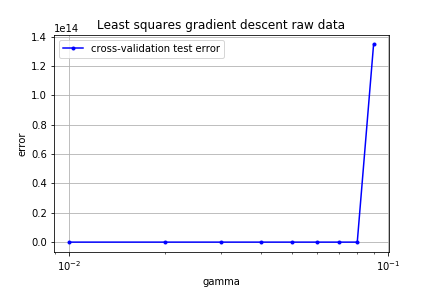
\includegraphics[width=0.4\textwidth]{plots/raw_data_least_squares_GD.png}
  \caption{Linear regression gradient descent}
  \label{fig:lsgd}
\end{figure}

\begin{figure}
  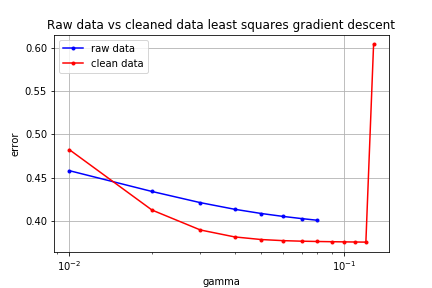
\includegraphics[width=0.4\textwidth]{plots/raw_vs_clean_lsgd.png}
  \caption{Raw vs cleaned data for LSGD}
    \label{fig:raw_clean_lsgd}
\end{figure}

\section{Ridge regression}
Daniel

\section{Logistic regression}
We also use cross-validation to test the efficiency of
\textit{logistic\_regression} on our standardized dataset.
We use five sets to set the hyperparameter $\gamma$.
For the initial weights chosen, they are all initialized to $0.5$ since $0.0, 0.1, ..., 0.6$ do not change the loss a lot but worsen the accuracy on AICrowd.
Our best submission with \textit{logistic\_regression} using raw data had an accuracy of $73.9\%$ and had 
\begin{lstlisting}
  max_iters = 1000
  k_fold = 5
  initial_weights = [0.5, 0.5, ..., 0.5]
  gamma = 1e-06
\end{lstlisting}
With cleaned data, the best submission has $72.7\%$ and use $\gamma = 1e-06$.
You can observe both in figure \ref{fig:raw_clean_log_reg}.

\begin{figure}
  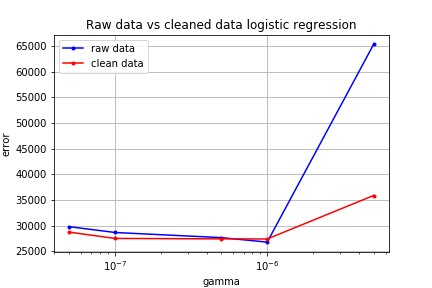
\includegraphics[width=0.4\textwidth]{plots/raw_vs_clean_log_reg.png}
  \caption{Raw vs cleaned data for logistic regression}
  \label{fig:raw_clean_log_reg}
\end{figure}


\section{Regularized logistic regression}
We implement cross-validation to optimize the values of $\lambda$ and $\gamma$. $\lambda$ takes values
$\{1,10,100,1000,10000\}$ and $\gamma$ takes values $\{10^{-6},10^{-7},10^{-8},10^{-9}\}$. Taking bigger
values for $\gamma$ results in the loss taking value $nan$. You can see the test error plotted against $\lambda$ in figure \ref{fig:raw_reg_log_regr}, each line corresponds to a value of $\gamma$. Other parameters are: 
\begin{lstlisting}
  max_iters = 3000
  k_fold = 3
  w_initial_raw = [0.0, 0.0, ..., 0.0]
\end{lstlisting}

This outputs the values for $\lambda$ and $\gamma$ that minimize the test error. These values are:
\begin{align*}
  \lambda &= 10 \\
  \gamma &= 10^{-6}
\end{align*}
Then we run the regularized logistic regression algorithm on the whole training with these two values but with $max\_iters = 30000$ to obtain a good $w$ vector.

\begin{figure}[h!]
  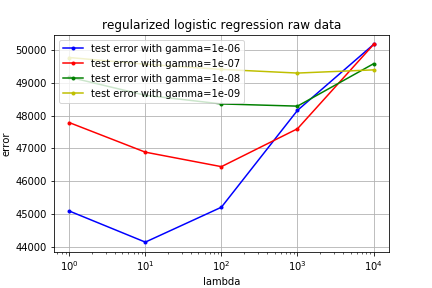
\includegraphics[width=0.5\linewidth]{plots/raw_data_reg_log_regr.png}
  \caption{Regularized logistic regression - HP optimization}
  \label{fig:raw_reg_log_regr}
\end{figure}

\end{document}
